\documentclass{beamer}

\usepackage[francais]{babel}
\usepackage[T1]{fontenc}
\usepackage[utf8]{inputenc}
\usepackage{beamerthemecs}
\usepackage{beamerouterthemecs}
\usepackage{beamerfontthemecs}
\usepackage{beamerinnerthemecs}
\usepackage{beamercolorthemecs}
\usepackage{hyperref}
  
\usetheme{cs}
\useoutertheme{cs}
\usefonttheme{cs}
\useinnertheme{cs}
\usecolortheme{cs}

\title[Les Réseaux Zigbee]{Les Réseaux Zigbee}
\author{\textbf{Thibault \textsc{Lengagne}, Sofian \textsc{Medbouhi} et Stanislas \textsc{Fechner}}}
\institute{Centrale Supélec - Campus de Rennes}

\begin{document}

  \begin{frame}
    \titlepage
  \end{frame}
  
  \AtBeginSection[] {
    \begin{frame}
      \frametitle{Plan}
      \tableofcontents[currentsection, hideothersubsections, pausesubsections]
    \end{frame} 
  }

\section{Introduction}

  \begin{frame}
     \frametitle{Stratégie}
	 \begin{block}{Zigbee est porté par la \textit{Zigbee Alliance}}
	    \begin{itemize}
		    \item créée en 2003
		    \item à l'époque sans concurrent important
		    \item désormais en compétition avec WeMo, Brillo et Thread (nous y reviendrons)
	    \end{itemize}
	    Les enjeux sont importants pour l'IoT. Applications à la domotique, contrôle industriel, smart cities...
	\end{block}
  \end{frame}

\begin{frame}
   \frametitle{Fonctions principales}

   \begin{block}{\textit{Zigbee} doit permettre de construire un réseau avec des équipements}
   \begin{itemize}
    \item de faible consommation (10mA reception, 19mA emission, 3uA hibernation)
    \item de faible débit/portée (100m)
    \item de faible puissance (de calcul)
   \end{itemize}
   Ce qui n'empêche pas le protocole d'implémenter AES128 notamment pour la payload
	\end{block}
  \end{frame}

    \begin{frame}
   \frametitle{Zigbee, IEEE 802.15.4}
   \begin{block}{Zigbee IEEE 802.15.4}
   \begin{itemize}
	   \item IEEE 802.15.4 définit les couches basses (physique et mac)
	   \item Zigbee définit les couches réseau et applicative
	   \item Cependant Zigbee fonctionne toujours sur 802.15.4, on confond souvent les deux..
   \end{itemize}
   \end{block}
  \end{frame}

 
  
 \section{La norme IEEE 802.15.4}
  \begin{frame}
    \frametitle{Zigbee et la norme 802.15.4}
    Le protocole Zigbee utilise ce protocole comme cadre de fonctionnement :
      \begin{center}
       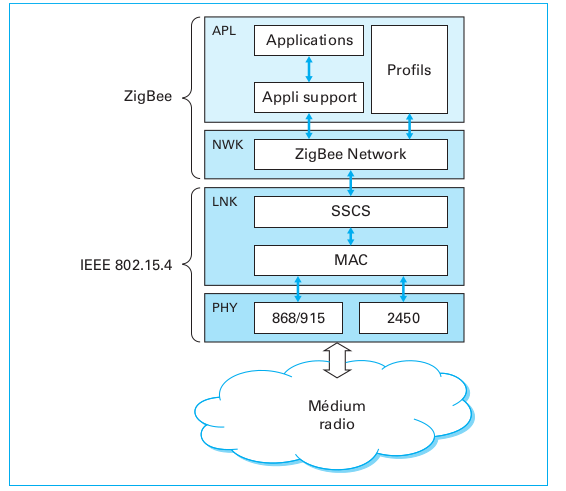
\includegraphics[scale=0.4]{OSI-Zigbee.png}
      \end{center}  
  \end{frame}

  \begin{frame}
    \frametitle{Comparatif}
    \begin{block}{Schema comparatif des différents protocole sans fil}
      \begin{center}
       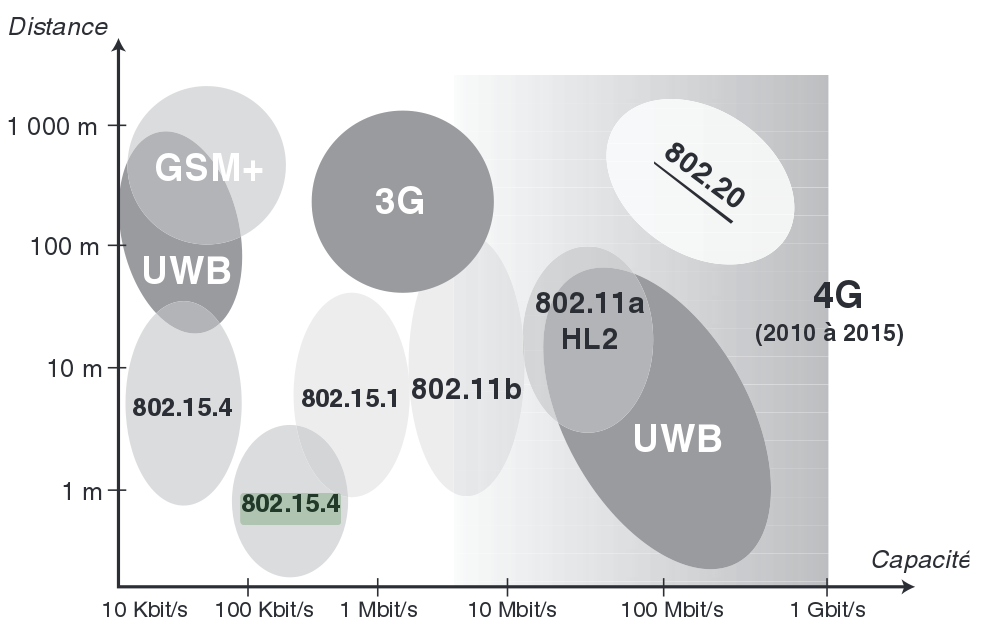
\includegraphics[scale=0.3]{Range.png}
      \end{center} 
    \end{block}
  \end{frame}
  
  \begin{frame}
    \frametitle{La couche physique}
    Contient l'émetteur/récepteur radio, avec un mécanisme de contrôle de qualité du signal et CCA
    \begin{block}{Débit}
      \begin{center}
       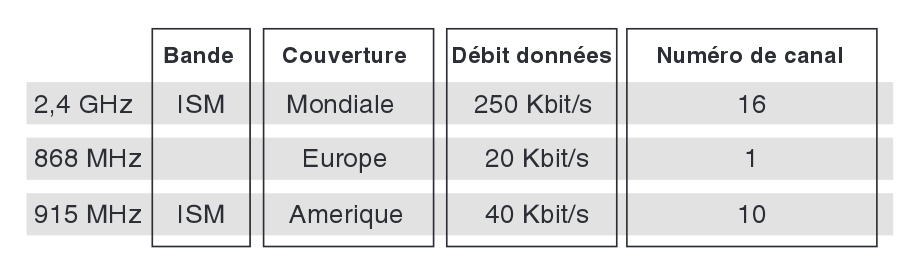
\includegraphics[scale=0.25]{Vitesse-Zigbee.png}
      \end{center}
    \end{block}
  \end{frame}
  
  \begin{frame}
    \frametitle{La couche d'accès au medium (MAC)}
    \begin{block}{Rôle des éléments du réseau}
      \begin{itemize}
        \item Le coordinateur (ZC) est le noeud principal, il est unique
        \item Les FFD ou routeurs gèrent le routage et les terminaux
        \item Les RFD ou terminaux sont de simple capteurs aux extremités du réseau
      \end{itemize}
    \end{block}
    \begin{center}
    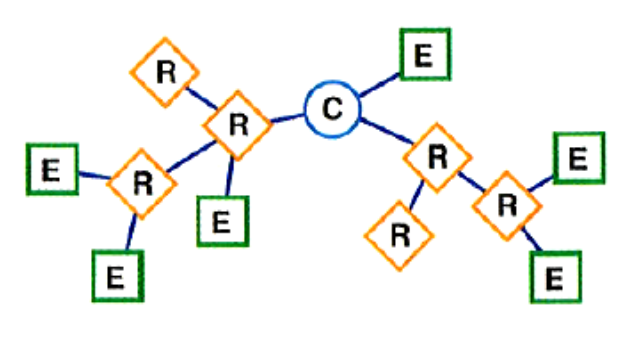
\includegraphics[scale=0.3]{Reseau.png}
    \end{center} 
  \end{frame}
  
  \begin{frame}
    \frametitle{La couche d'accès au medium (MAC)}
    \begin{block}{Format de trame}
      \begin{itemize}
        \item En-tête (contrôle de trame, numéro de séquence, adressage)
        \item Données
        \item Pied (CRC)
        \begin{center}
         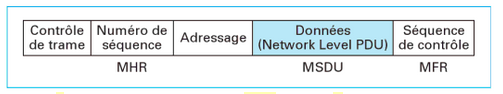
\includegraphics[scale=0.6]{Couche-MAC.png}
        \end{center} 
      \end{itemize}
    \end{block}
  \end{frame}
  
  \begin{frame}
    \begin{block}{Il existe deux modes de fonctionnement}
      \begin{itemize}
        \item Le mode non-coordonnée, ou \textit{non-beacon}
        \item Le mode coordonnée, ou balisé, ou\textit{beacon}
      \end{itemize}
    \end{block}
  \end{frame}

  
  \begin{frame}
    \frametitle{La couche d'accès au medium (MAC)}
    \begin{block}{Le mode non-Coordonnée}
      \begin{itemize}
        \item Pas d'emission de \textit{beacon}
        \item Fonctionnement CSMA/CA pour gérer les collisions
        \item Le coordinateur est éveillé en permanence
      \end{itemize}
    \end{block}
  \end{frame}

  \begin{frame}
    \frametitle{La sous-couche d'accès au medium (MAC)}
    \begin{block}{Le mode Coordonnée}
      Le coordinateur diffuse périodiquement des \textit{beacon}. Tous les dispositifs sont informés de :
      \begin{itemize}
        \item La durée de la \textit{superframe} et quand ils peuvent transmettre des données en CSMA/CA
        \item A partir de quel moment le coordinateur rentre en hibernation et pour quelle durée
        \item Tous les dispositifs se réveillent quelques instants avatn l'emission du \textit{beacon}
      \end{itemize}
    \end{block}
  \end{frame}
  
  \begin{frame}
    \begin{center}
    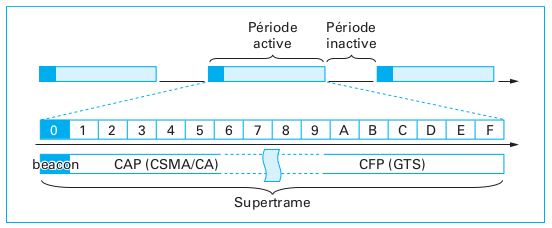
\includegraphics[scale=0.6]{Supertrame.png}
    \end{center} 
  \end{frame}


  \begin{frame}
    \frametitle{La sous-couche de convergence (LLC)}
    \begin{block}{A la sous-couche MAC est ajouté une sous-couche de convergence LLC}
    \begin{itemize}
      \item Vérification de l'intégrité des données reçues (CRC)
      \item Contrôle de flux, afin d'éviter la saturation
      \item La convergence d'adressage (correspondance couche 2 et 3 du modèle OSI, gestion du broadcast et en multicast)
    \end{itemize}
    \end{block}
  \end{frame}

  \section{Le protocole ZigBee - Couche réseau et applicative}

  \begin{frame}
   \frametitle{Noeuds du réseau}
   \begin{block}{Un réseau Zigbee contient trois types de noeuds}
      \begin{itemize}
	\item \textbf{ZigBee Coordinator} : unique dans le réseau, la création du réseau s'articule autour de lui. Lorsque le réseau est crée, il se comporte comme un noeud routeur
	\item \textbf{ZigBee Router} : participe au routage, mais peut également envoyer et recevoir des messages
	\item \textbf{ZigBee End Device} : noeud le plus simple du réseau. Il n'est qu'un élément final et ne participe pas au routage des messages
      \end{itemize}
    \end{block}	
  \end{frame}
  
  \begin{frame}
   \frametitle{Formation du réseau}
   \begin{block}{La création du réseau démarre en installant le premier noeud, qui joue le rôle de coordinateur}
    \begin{itemize}
     \item Le réseau est identifié par un canal et un identifiant de réseau. Cela permet à plusieurs réseau d'utiliser le même canal
     \item Un noeud recherche un réseau en scannant les canal autour de lui
     \item Lorsqu'il souhaite intégrer le réseau, il envoie une demande de connexion au noeud routeur le plus proche de lui 
    \end{itemize}
   \end{block}
  \end{frame}

  
  \begin{frame}
   \frametitle{Topologie du réseau}
   \begin{block}{Plusieurs type de topologies sont envisageable}
   \begin{columns}
    \column{0.6\textwidth}
    \begin{itemize}
     \item \textbf{Topologie en arbre} : les noeuds qui le peuvent se connectent au coordinateur, et les noeud trop éloignés se connectent au routeur le plus proche
     \item \textbf{Topologie maillée} : tous les noeuds routeurs à porté les uns des autres peuvent communiquer entre eux. Les noeuds terminaux ne sont connectés qu'à un routeur
    \end{itemize}
    \column{0.4\textwidth}
    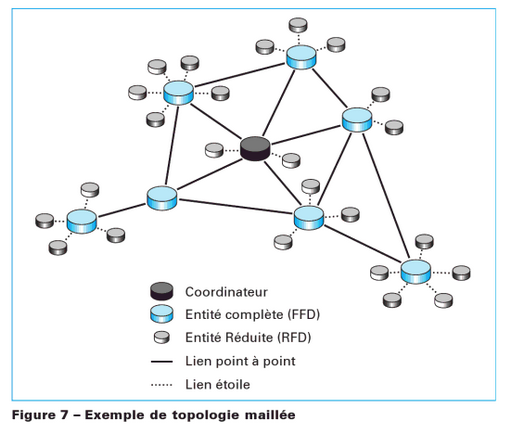
\includegraphics[scale=0.25]{Topologie-Maille.png}
   \end{columns}
   \end{block}
  \end{frame}
  
  \begin{frame}
    \frametitle{Adressage}
    \begin{block}{ZigBee autorise deux type d'adressages différents}
      \begin{itemize}
	\item \textbf{Adressage libre} : l'addressage est determiné par le profil applicatif
	 \item \textbf{Adressage en arbre} : Zigbee propose un algorithme de distribution d'adresses automatique. Cet algorithme suit l'arborescence du réseau autour du coordinateur
	 \begin{itemize}
	  \item Décentralisé, ce qui minimise les échange au sein du réseau pour attribuer une nouvelle adresse
	  \item Unicité des adresses
	  \item Facilite le routage des messages
	 \end{itemize}

      \end{itemize}     
    \end{block}
  \end{frame}
  
  \begin{frame}
    \frametitle{Routage}
    \begin{block}{Selon le type d'addressage utilisé, deux protocoles de routage peuvent être utilisés}
      \begin{itemize}
        \item \textbf{Routage à la demande} : le noeud vérifie sa table de routage. Soit il trouve une entrée correspondante à sa destination et transmet le message, sinon il diffuse une requète de demande de route. Cette requète de route atteint le noeud destinataire, qui répond en renvoyant un message qui emprunte la route inverse. Ce message atteint le noeud emetteur, qui peut alors envoyer son message en suivant cette route
        \item \textbf{Routage hiérarchique} : valable uniquement pour l'adressage en arbre. Ce type d'adressage étant deterministe, il est possible de determiner à quel voisin transmettre le message pour atteindre le noeud final
      \end{itemize}
    \end{block}
  \end{frame}
  
  \begin{frame}
   \frametitle{Couche Applicative}
   \begin{block}{ZigBee propose plusieurs profils adaptés à différents usages}
     \begin{itemize}
      \item \textbf{Gestion de bâtiments} : contrôle des accès, de l'éclairage, du chauffage
      \item \textbf{Périphérique électronique} : clavier ou souris sans fil, télécommande
      \item \textbf{Médical} : suivi des patients, monitioring des activités du corps humain pendant un effort physique
     \end{itemize}
     
     Chacun de ces profils est en fait un protocole qui determine la nature des messages a transmettre afin de faire fonctionner le réseau

   \end{block}

  \end{frame}
  
  \begin{frame}
  \frametitle{La sécurité chez Zigbee ?}
  \begin{block}{Implémente une variation de AES-CCMP}
    \begin{itemize}
	\item Clé de 128 bits
	\item MIC de longueur variable
	\item 3 variations : 'link key" "network key", "master key" (pro)
	\item diffusion des clés : OTA/flashage
    \end{itemize}
  Chiffrement symétrique basé sur un chiffrement conforme au RGS
  \end{block}
  \end{frame}

  \begin{frame}
  \frametitle{La sécurité chez Zigbee ?}
  \begin{block}{Cependant deux failles majeures}
    \begin{itemize}
	\item la clé est diffusée en plaintext
	\item limitations importantes : révocation, durée de vie
    \end{itemize}
  \end{block}
  \begin{block}{Ce qui nous amène à des attaques fonctionnelles concrètes}
  \begin{itemize}
      \item Sniffer la  clé
      \item Attaques de type replay
      \item Aide des constructeurs : clé dans le firmware, encore plus mauvaises implémentations, etc..
  \end{itemize}
  Un framework comparable (dans l'idée) à aircrack existe déjà : killerbee
  \end{block}
  \end{frame}

  
  \section{Conclusion}

  \begin{frame}
    \frametitle{Conclusion}
    \begin{block}{Zigbee est toujours le protocole de référence :}
      \begin{itemize}
	\item Porté par un consortium à la différence de Thread/Brillo (Google) Homekit (Apple) WeMo (Belkin), composé de Phillips/TexasInstrument/Schneider/NXP...
	\item Connu depuis longtemps d'où 75\% des parts de marché
	\item Possibilité pour les constructeurs de modifier les "profils Zigbee" i.e enrichir la couche applicative
	\item protocole en évolution constante : Zigbee 3.0 en développement
      \end{itemize}  
    \end{block}
  \end{frame}
  

  \begin{frame}
    \frametitle{Conclusion}
    \begin{block}{Cependant quelques écueils qui pourraient se révéler graves}
      \begin {itemize}
	\item Non compatible avec IP à la différence de 6LowPAN (sur lequel est basé Thread), ces protocoles devraient représenter 35\% des ventes en 2019 (2\% ajdh)
	\item Une force est une faiblesse : pas d'entité unique qui porte le standard 
	\item De même les profils différents sont mal utilisés : amènent à des incompatibilités
	\item Des problèmes liés à la sécurité
	\begin{itemize}
	  \item Le réseau contient des noeuds à communication chiffrés, d'autres non, attaque MitM
	  \item Attaques restreintes (faible puissance de calcul)
	  \item Mais à venir !
	\end{itemize}
      \end{itemize}
    \end{block}
  \end{frame}  

\end{document}
